\begin{frame}[t]{Морфология на невроните}
  \begin{enumerate}
    \item   Дендрити - разклонявания на клетната, в краищата на които бива въздействана от други неврони
    \item   Сома - "основната" част на клетката, включваща ядрото и повечето органели
    \item   Аксон - къс (в ЦНС) или дълъг (в ПНС) израстък, служещ за предаване на импулси към други клетки
    \item   Телодендрия - разколявания на аксона в края му
    \item   Синапс - окончание на разклоненията. 
    \begin{enumerate}
      \item   Електрични синапси - сдвояване на клетки
      \item   Химични синапси - контакът се извършва непряко чрез невротрансмитери
    \end{enumerate}
    \item   Прищъпване на Ранвие - участък между два миелинови участъка
  \end{enumerate}
\end{frame}

\begin{frame}[t]{Морфология на невроните}
  \begin{figure}[htbp!]
    \centering
    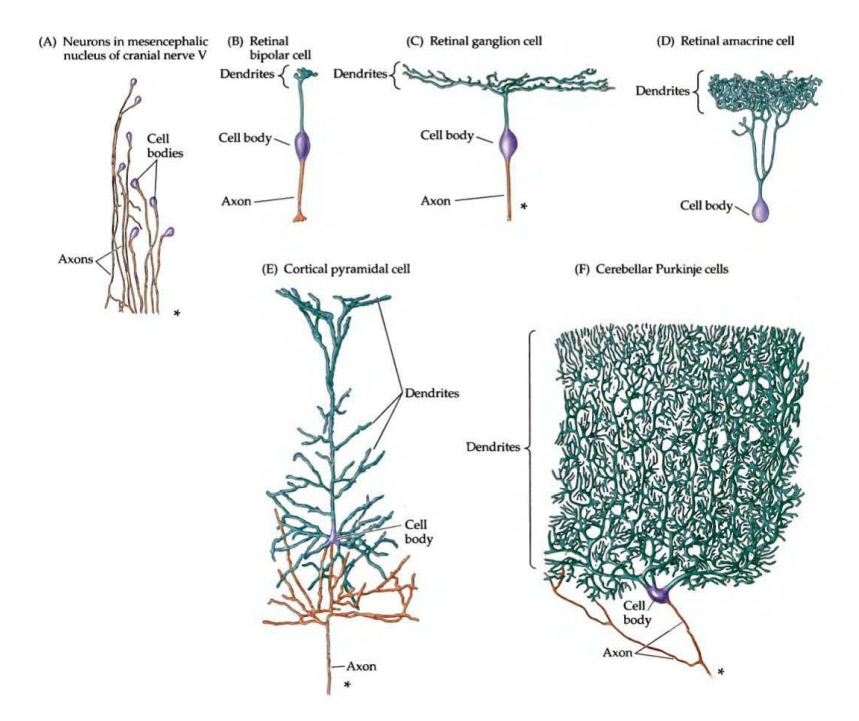
\includegraphics[width=\textwidth,height=0.7\textheight,keepaspectratio]{neuron-types.PNG}
    \caption{Фиг 1.2 от Neuroscience}
  \end{figure}
\end{frame}

\begin{frame}[t]{Морфология на невроните}
  \begin{figure}[htbp!]
    \centering
    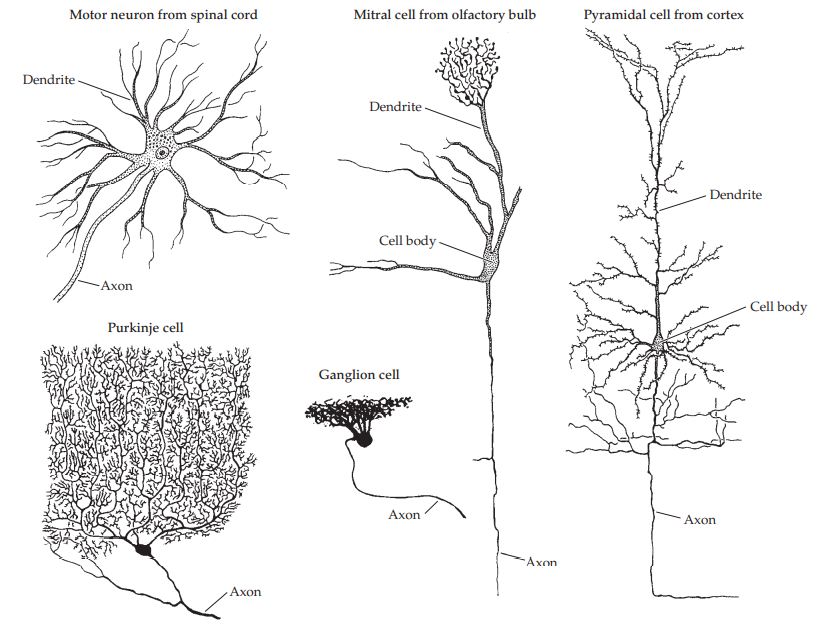
\includegraphics[width=\textwidth,height=0.7\textheight,keepaspectratio]{neuron-types-2.PNG}
    \caption{Фиг 1.4 от From Neuron to Brain}
  \end{figure}
\end{frame}

\begin{frame}[t]{Морфология на невроните}
  \begin{figure}[htbp!]
    \centering
    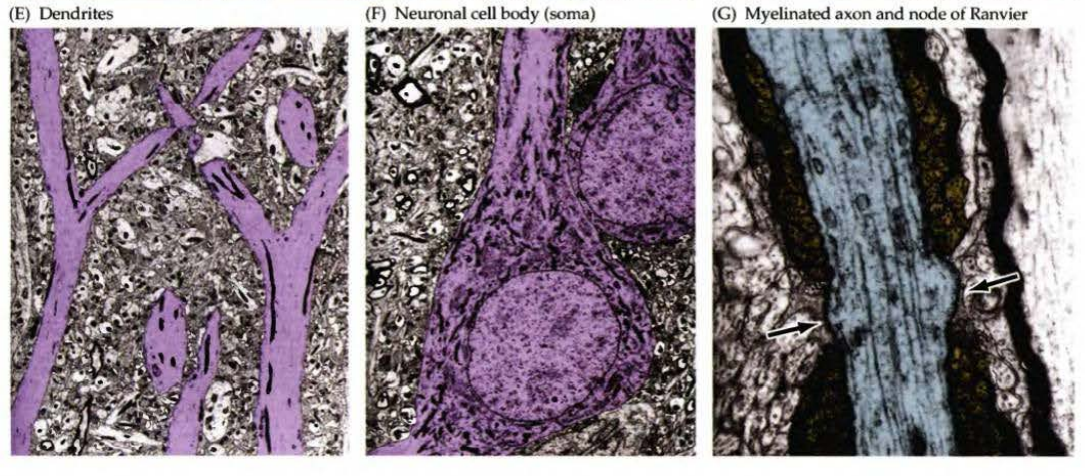
\includegraphics[width=\textwidth,height=\textheight,keepaspectratio]{neuron-parts.PNG}
    \caption{Дендрити, сома и аксон Фиг 1.3 от Neuroscience}
    \label{figure:usf}
  \end{figure}
\end{frame}

